%% LyX 2.3.0 created this file.  For more info, see http://www.lyx.org/.
%% Do not edit unless you really know what you are doing.
\documentclass{article}
\usepackage[T1]{fontenc}
\usepackage[latin9]{inputenc}
\usepackage{geometry}
%\geometry{verbose,tmargin=2.5cm,bmargin=2.5cm,lmargin=2.5cm,rmargin=2.5cm,headheight=1.5cm,headsep=1.5cm,footskip=1.5cm}
\usepackage{color}
\usepackage{babel}
\usepackage{refstyle}
\usepackage{float}
\usepackage{amsmath}
\usepackage{amsthm}
\usepackage{amssymb}
\usepackage{stmaryrd}
\usepackage{setspace}
\usepackage{comment}
\usepackage{mathtools}

\usepackage[unicode=true,pdfusetitle,
 bookmarks=true,bookmarksnumbered=false,bookmarksopen=false,
 breaklinks=false,pdfborder={0 0 1},backref=false,colorlinks=true]
 {hyperref}

\usepackage[colorinlistoftodos]{todonotes}


\makeatletter

%%%%%%%%%%%%%%%%%%%%%%%%%%%%%% LyX specific LaTeX commands.

\AtBeginDocument{\providecommand\corref[1]{\ref{cor:#1}}}
\AtBeginDocument{\providecommand\thmref[1]{\ref{thm:#1}}}
\AtBeginDocument{\providecommand\lemref[1]{\ref{lem:#1}}}
\AtBeginDocument{\providecommand\figref[1]{\ref{fig:#1}}}
%% Because html converters don't know tabularnewline
\providecommand{\tabularnewline}{\\}
\RS@ifundefined{subsecref}
  {\newref{subsec}{name = \RSsectxt}}
  {}
\RS@ifundefined{thmref}
  {\def\RSthmtxt{theorem~}\newref{thm}{name = \RSthmtxt}}
  {}
\RS@ifundefined{lemref}
  {\def\RSlemtxt{lemma~}\newref{lem}{name = \RSlemtxt}}
  {}


%%%%%%%%%%%%%%%%%%%%%%%%%%%%%% Textclass specific LaTeX commands.
\theoremstyle{plain}
\newtheorem{thm}{\protect\theoremname}
\theoremstyle{definition}
\newtheorem{defn}[thm]{\protect\definitionname}
\theoremstyle{plain}
\newtheorem{cor}[thm]{\protect\corollaryname}
\theoremstyle{remark}
\newtheorem*{note*}{\protect\notename}
\theoremstyle{remark}
\newtheorem*{rem*}{\protect\remarkname}
\theoremstyle{remark}
\newtheorem*{notation*}{\protect\notationname}
\theoremstyle{remark}
\newtheorem{claim}[thm]{\protect\claimname}
\theoremstyle{plain}
\newtheorem{lem}[thm]{\protect\lemmaname}
\theoremstyle{plain}
\newtheorem{prop}[thm]{\protect\propositionname}

%%%%%%%%%%%%%%%%%%%%%%%%%%%%%% User specified LaTeX commands.
\usepackage{tikz}
\newref{claim}{name=claim~}
\newref{cor}{name=corollary~}
\providecommand{\thmautorefname}{Theorem}
\providecommand{\corautorefname}{Corollary}
\providecommand{\lemautorefname}{Lemma}
\providecommand{\claimautorefname}{Claim}

\makeatother

\providecommand{\claimname}{Claim}
\providecommand{\corollaryname}{Corollary}
\providecommand{\definitionname}{Definition}
\providecommand{\lemmaname}{Lemma}
\providecommand{\notationname}{Notation}
\providecommand{\notename}{Note}
\providecommand{\propositionname}{Proposition}
\providecommand{\remarkname}{Remark}
\providecommand{\theoremname}{Theorem}
\newcommand{\FF}{\mathsf{F}}
\newcommand{\ff}{\mathsf{f}}
\newcommand{\N}{\mathbb{N}}
\newcommand{\Z}{\mathbb{Z}}
\newcommand{\cF}{\mathcal{F}}
\begin{document}

\title{Firefighting on skyscrapers}
\date{\today}

\maketitle

\section{Introduction}

Let $G=\left(V,E\right)$ be an infinite graph. 
The firefighter problem is the following combinatorial solitaire game introduced by Hartnell \textcolor{red}{(ADDREF)}: 
We begin with a finite starting set of \emph{burning} vertices $S\subseteq V$. At every timestep $t\in\mathbb{N}$, the player choose an arbitrary finite collection of $f(t)$ non burning vertices and \emph{protects} them permanently. Then, at time $t+\frac{1}{3}$ all the unprotected neighbors of burning vertices become burning and the process continues ad infinitum. If at some timestep no new burning vertices
are generated, we say that the player \emph{contained} the fire.

Consider the graphs $\Z\boxempty \Z$ whose vertices consist of the integer two dimensional lattice $Z^2$ with 
$L_1$ nearest neighbour adjacency and $\Z \boxtimes \Z$ on the same lattice with $L_\infty$ nearest neighbour adjacency.
In \cite{FH} Hod and the second author, investigated for which $f$ for any starting fire $S$ the player has a strategy that allows him to eventually contain the fire. Here we investigate the same problem on the graphs 
$G\in\{\Z\boxempty\Z\boxempty[h], \Z\boxtimes\Z\boxtimes[h]\}$, which consist of a slab $\Z\times\Z\times\{1,\dots, h\}$ in $\Z^3$, with the corresponding connectivities.



For every $\ff:\N\rightarrow\N$, look at the
family of strategies $\cF\left(\mathsf{f}\right)$ such that at step $t$ the player protect at most $\mathsf{f}\left(f\right)$ vertices\todo{O: Either "at most" or rounded. Also not consistent with notation later, see remark in the theorem.}. We say that $\mathsf{f}$ \emph{contains} the fire if for all finite $S$ there is a strategy in $\mathcal{F}\left(\mathsf{f}\right)$
such that the fire is bounded (note here that $\boxempty$  and $\boxtimes$ are the Cartesian product,  and  the strong Cartesian product of graphs, respectively).

%Let $G$ be a graph, one can ask for optimal $\mathsf{f}$ in some
%sense that depends on the growth of $G$, for example, for $\Z\boxempty\Z$
%any $\mathsf{f}\left(t\right)\equiv c$ with $\frac{3}{2}<c$ contains the
%fire and $\mathsf{f}\equiv\frac{3}{2}$ is not enough \cite{key-1}\todo{You mean that for every such f the fire could be contained. f is not a strategy.}\todo{A: We define the term "contain" to be an attribute of a function}. The optimal $\mathsf{f}$ is known for a few graphs and there are bounds
%for the limit behavior for a lot of graphs, in particular for Cayley
%graph with polynomial and intermediate growth \cite{key-3}.

%This paper generalize the Cartesian result by proving that $\mathsf{f}\equiv\frac{3}{2}h$
%is the right function for containment in $G=\mathbb{Z}\boxempty\mathbb{Z}\boxempty L_{h}$.

%Let $h\in\mathbb{N}$, denote by $L_{h}$ the segment of length $h$,
%which is the graph with $V=\left[h\right]$ and 
%\[
%E=\left\{ \left(a,b\right)|\left|a-b\right|=1\right\} .
%\]


\begin{thm}
\label{thm:1}For every $h\in\mathbb{N}$, let $G_{h}=\mathbb{Z}\boxempty\mathbb{Z}\times L_{h}$.
Let $\frac{3}{2}<c$ then $\mathsf{f}\left(t\right)\equiv ch$ contains
the fire, and $\mathsf{f}\equiv\frac{3}{2}h$ are not enough.
\end{thm}

\begin{thm}
\label{cor:2}For every $h\in\mathbb{N}$, let $G_{h}=\mathbb{Z}\boxtimes\mathbb{Z}\times L_{h}$.
Let $3<c$ then $\mathsf{f}\left(t\right)\equiv ch$ contains the fire,
and $\mathsf{f}\equiv 3h$ are not enough.
\end{thm}
\textcolor{red}{remarks about stronger results that we obtain or could obtain.}
\subsection{Background}
\subsection{Discussion and open problems}
\subsection{Proof outline + outline of the paper}

\section{Preliminaries}

To make the description of the problem exact, we
define the timeline of the game:
\begin{center}
\begin{tabular}{|c|c|c|}
\hline 
time & event & updated quantity\tabularnewline
\hline 
\hline 
$-\frac{1}{3}$ & The initial fire created & $B(0)$ is set\tabularnewline
\hline 
$t+\frac{1}{3}$ & Protected vertices are selected & $F(1)\setminus B(0)$ are protected\tabularnewline
\hline 
$t+\frac{2}{3}$ & fire spreads to unprotected adjacent vertices& $B(t+1)$ is determined\tabularnewline
\hline 
$t$ & Nothing &\tabularnewline
\hline 
\end{tabular}
\par\end{center}

Denote the four axis aligned directions by $e_{0}=\left(0,1\right)=-e_{2},e_{1}=\left(1,0\right)=-e_{3}$.
Call the sub-lattice $\Z^2\times\{k\}$ the $k$-th \emph{level} of our graph. 
Throughout, we follow the convention that level is given in the superscript and direction is given in the subscript.
Addition in subscript indices is always taken modulo 4.
Denote the graph distance between vertices $v,u$ by $d(v,u)$ and write $S^+=\{v\ :\ d(v,S)\le 1\}$.

Given $\FF\left(t\right), B(0) \subseteq\mathbb{Z}^{2}\times\left[h\right]$ we inductively define $B_{\FF}(t)=B\left(t\right),\FF\left(t\right)$ for $t\in\N$ by
$$B(t)=B(t-1)\cup \left(B(t-1)^+\setminus \FF(t)\right).$$
Observe that here we allow $\FF(t)$ to overlap with $B(t-1)$, however, such overlapping elements have no effect on the evolution of $B(t)$. 
The reader may think of $\FF(t)$ as the orders of the player concerning which vertices to protect, so that illegal orders are simply ignored.
$B(t)$ describes the evolution of the burning vertices so that $B(t)$ are the vertices burning at time $t$
and $\FF(t)\setminus B(t)$ are the vertices protected just before the fire spread at time $t-\tfrac{1}{3}$. 

\textcolor{red}{Where to put and how to improve:}
In our proof for the lower bound on the asymptotic rate of protected vertices needed to contain the fire, we are interested only in new burning vertices. This observation led the authors of \cite{FH} to consider only \emph{firefronts} - the burning vertices at time $t$ which are most distant in a certain direction from a point in the starting set of burning vertices. Here we develop this idea further, keeping track of a \emph{fronts structure}, the intersection of $B(t)$ with a certain a sets, chosen so that 
as long as this set keeps moving away from the origin, the fire is not contained. (two main changes - a. fronts move in a multilayer form, so that sometimes a level moves without having any fire on, b. fronts may sometime not move, even though there is more distant fire in that direction.)

\subsection{the fronts structure}

Call an vector $\{x_k\}_{k\in[h]}\in \N^h$ \emph{Lipschitz} if $|x_{k+1}-x_{k}|  \le 1$ for all $k\in (0,\dots,h-1)$.
\begin{defn}
Given $\rho = (r^1_{i},\dots,r^h_{i})_{i\in[4]}$, four Lipschitz vectors, define a
\emph{fronts structure} of $\rho$ as $(L_0,L_1,L_2,L_3)$
$$L_i(\rho)=\bigcup_{k\in[h]}\{r^h_i e_i+a e_{i+1}\ :\ a\in \{-r^h_{i-1}+1,\dots,r^h_{i+1}-1\} \},$$
\todo{verify the sign of a}
\todo{3D figure of Lipschitz vector - $L_{i}$}
writing
$$L^k_i(\rho)=L_i(\rho)\cap (\Z^2\times\{k\}),$$
\end{defn}
\begin{comment}
\begin{defn}
For all $i\in\left[4\right],k\in\left[h\right]$ define, $r_{i}^{k}\left(t\right)$
- the \emph{fire range} in the i-th direction and the k-th
level inductively and $r_{i}^{k}\left(0\right)$ can be choose arbitrary.

Define
\[
r_{i,j}^{k}\left(t\right)=\left(e_{i}r_{i}^{k}\left(t\right)+e_{j}r_{j}^{k}\left(t\right)\right)\times\left\{ k\right\} \in V,
\]
\end{defn}
\end{comment}

which is the i-th j-th corner.


\begin{defn}
The i-th \emph{firefront} of the k-th \emph{level} is
\[
L_{i}^{k}\left(t\right)=\left\{ ur_{i,i+1}^{k}\left(t\right)+\left(1-u\right)r_{i,i-1}^{k}\left(t\right)|u\in\left[0,1\right]\right\} \cap\mathbb{Z}^{3}\setminus\left\{ r_{i,i+1}^{k}\left(t\right),r_{i,i-1}^{k}\left(t\right)\right\} \subseteq V.
\]
For example 
\[
L_{1}^{k}\left(t\right)=\left\{ \left(r_{1}^{k}\left(t\right),y,k\right)|y\in\mathbb{Z},-r_{2}^{k}\left(t\right)<y<r_{0}^{k}\left(t\right)\right\} 
\]
 (the other fronts have $r_{i}^{k}\left(t\right)$ in the y coordinate
or negative sign).
\end{defn}

\begin{cor}
\label{cor:1} For every distinct pair $(i,k)\neq (j,\ell)$ we have
$$ L_{i}^{k}(t)\cap L_{j}^{\ell}(t)= \varnothing $$
\end{cor}
\begin{proof}
Observe that $r_{1}^{k}\left(t\right)$ is greater then the $x$ coordinate of points in $L_{0}^{k}(t)$ and equals the x coordinate of points in  $L_{1}^{k}(t)$, use the same arguments for any disjoint pair $(i,j)$. For disjoint pair of $(k,\ell)$, looking at the $z$  coordinate completes the proof. 
\end{proof}


The rules of the firefighter problem are:
\[
B\left(t+1\right)=B\left(t\right)\cup B\left(t\right)^{+}\setminus F\left(t+1\right).
\]

Useful method is to make a time change to the fire and the firefighters
and count them in ``frontal time''. To do so, we have the following
definition.
\begin{defn}
The $potential$ \todo{A: The "fire volume of the front"? but I think that "frontal fire" are the points, maybe: "The potential of the frontal fire" is: $\varphi$ ... from now on call "the potential". maybe: firocity} is:
\[
\varphi_{i}^{k}\left(t\right)=\left|L_{i}^{k}\left(t\right)\cap B\left(t\right)\right|.
\]
\end{defn}

\begin{defn}
Denote
\[
\mathsf{F}_{i}^{k}\left(t\right)=\left(F\left(t\right)\cap L_{i}^{k}\left(t\right)\right)\setminus\mathsf{F}_{i}^{k}\left(t-1\right),
\]

which are the new firefighters on level k and front i at time t. Denote
\[
f_{i}^{k}\left(t\right)=\left|\mathsf{F}_{i}^{k}\left(t\right)\right|.
\]
\end{defn}

\begin{rem*}
From now on the paper uses only $f$ and the assumption $\mathsf{f}\left(t\right)=ct$
equivalent to $\left|F\left(t\right)\right|\leq ct$.
\end{rem*}
\begin{cor}
For all $t\in \mathbb{N}$ we have $$\sum_{i\in \left[4\right]}\sum_{k\in\left[h\right]}\sum_{\tau=1}^{t}f_{i}^{k}\leq\left|F\left(t\right)\right|.$$
\end{cor}
\begin{proof}
Let $t\tau<t$, by induction: $\mathsf{F}_{i}^{k}\left(t\right)\cap\mathsf{F}_{i}^{k}\left(\tau \right)=\varnothing$.
\corref{1} shows the disjointness of $L_{i}^{k}\left(\tau\right),L_{j}^{\ell}\left(\tau\right)$
for distinct pairs of $\left(i,j\right),\left(k,\ell\right)$ conclude
that
\[
\sum_{i\in \left[4\right]}\sum_{k\in\left[h\right]}\sum_{\tau=1}^{t}f_{i}^{k}\leq\left|F\left(t\right)\right|.
\]
\end{proof}


%Arye: maybe summing on i,k together, like that:
%\sum_{i\in \left[4\right],k\in\left[h\right]}\sum_{\tau=1}^{t}f_{i}^{k}\leq\left|F\left(t\right)\right|.


\begin{notation*}
Unless mentioned else, this paper uses the following summation notations:
``missing'' index meaning summation on this index, for example $v_{i}:=\sum_{k\in\left[h\right]}v_{i}^{k}$,
summation of objects with different index denoting by subset of the
indices , for example $v_{\left\{ i,j\right\} }^{k}:=v_{i}^{k}+v_{j}^{k}$.
Summation up to $t$ will be denoted by upper asterisk , for example $f\left(t\right)^{\ast}=\sum_{i\in \left[4\right]}\sum_{k\in\left[h\right]}\sum_{\tau=1}^{t}f_{i}^{k}\left(\tau\right)$ and $\varphi(t)=\sum_{i\in[4]}\sum_{k\in[h]}\varphi_i^k(t)(=\left|\bigcup_{i\in[4],k\in[h]} L_i^k(t)\cap B(t)\right|$)
\end{notation*}

To obtain some properties of the fire and the distance we need a ''fronts structure''.
\begin{defn}
Similar to $r_{i}^{k}\left(t\right)$ , define $\alpha_{i}^{k}\left(t\right)$
inductively. 
\[
\alpha_{i}^{k}\left(t+1\right)=\begin{cases}
6h^{2}\left(r_{i}^{k}\left(t\right)-r_{i}^{\min}\left(t\right)+1\right) & g_{i}\left(t\right)=0\\
2h\left(r_{i}^{k}\left(t\right)-r_{i}^{\min}\left(t\right)+1\right) & g_{i}\left(t\right)=1
\end{cases},
\]
\end{defn}

where $r_{i}^{\min}\left(t\right)=\min_{k\in\left[h\right]}r_{i}^{k}\left(t\right)$.
Think on $\alpha_{i}^{k}\left(t\right)$ as the threshold of letting
the fire in the i-th front ,k-th level move forward while preserving
the frontal structure.

The function $g_{i}\left(t\right)$ indicates whether the amount of fire
in time $t$ is greater then expected, by looking at the symmetric
toy model, and will define later in this paper.
\begin{defn}
Define 
\[
a_{i}^{k}\left(t\right)=1_{\varphi_{i}^{k}\left(t\right)>\alpha_{i}^{k}\left(t\right)},
\]
which indicate if the k-th level is \emph{spreading}.

The k-th level is $pulled$ if there is a spreading level, $\ell\ne k$
with:
\[
r_{i}^{\ell}\left(t\right)-r_{i}^{k}\left(t\right)\geq\left|\ell-k\right|.
\]
\end{defn}

\begin{defn}
The difference in the distance denoted by $\Delta r_{i}^{k}\left(t\right):=r_{i}^{k}\left(t+1\right)-r_{i}^{k}\left(t\right)$
equals 1 if the level is spread or pulled, and 0 otherwise.
\end{defn}

%\begin{comment}
%%re-writing the introducing of r
Discussion: let $\{r_i^k(t)\}$ be a vector with the following properties:
\begin{itemize}
    \item $\{r_i^k(t)\}$ is a Lipschitz vector
    \item $a_i^k(t)=1$ implies $r_i^l(t)=1$
    \item \textcolor{red}{May we include property of being
    pulled?, we can't allow $r_i^k$ to move if the front is non-active}
    \item \textcolor{red}{ and we must have  $r_i^k(t)-r_i^k(t+1)\in {0,1}$ otherwise we have some Fogarty's proof problems}
\end{itemize}
One way to maintain fronts structure with these properties is by setting the fire-range as following: first $a_i^k(t)=1$ implies $\Delta r_i^k(t)=1$ which guarantee the first property, second if there is $k$ with  $r_i^{k-1}(t)+1=r_i^{k}(t)$ and $a_i^k(t)=1$ then setting $\Delta r_i^{k-1}(t)=1$ (and maybe $\Delta r_i^{k-2}(t)=1$ and so on) will guarantee the second property. Otherwise set $\Delta r_i^k(t)=0$. formally writing: 
\[
\Delta r_i^k(t)= \begin{cases*}
1 & $\exists$ $0\le d$, $r_i^{d+k}(t)=r_i^k(t)+d$, $a_i^{k+d}(t)=1$ \\
0 & Otherwise
\end{cases*}
\]
\begin{cor}
Indeed $\{r_i^k(t)\}_{k\in[h]}$ is a Lipschitz vector
\end{cor}
\begin{proof}
By induction, assume $\{r_i^k(t)\}_{k\in[h]}$ is a Lipschitz vector. The non trivial case happen when $r_i^{k}(t)=r_i^{k-1}(t)+1$, $\Delta r_i^k(t)=1$ and $a_i^k(t)=0$, in this case there is $d$ with $r_i^{d+k}(t)=r_i^k(t)+d$ and $a_i^{k+d}(t)=1$, deduce that $r_i^{d+k}(t)=r_i^{k-1}(t)+d+1$, therefore, $d+1$ is a witness to the fact that $\Delta r_i^{k-1}(t)=1$ and $\{r_i^k(t+1)\}_{k\in[h]}$ is a Lipschitz vector.
\end{proof}


%\end{comment}

One of the properties of the frontal structure is presented in the
following claim.
\begin{claim}
For all $t\in\mathbb{N},k\in\left\{ 1,...h-1\right\} $ we have $\left|r_{i}^{k+1}\left(t\right)-r_{i}^{k}\left(t\right)\right|\leq1$.
\end{claim}

\begin{proof}
By induction, assume the lemma holds for $t$ and without loss of
generality $r_{i}^{k}\left(t\right)\leq r_{i}^{k+1}\left(t\right)$,
in fact assume that $r_{i}^{k}\left(t\right)<r_{i}^{k+1}\left(t\right)$
since, by $\left|\Delta r_{i}^{k}\left(t\right)\right|\leq1$, the
case $r_{i}^{k}\left(t\right)=r_{i}^{k+1}\left(t\right)$ is trivial.
Use the hypothesis to write $r_{i}^{k}\left(t\right)+1=r_{i}^{k+1}\left(t\right)$, assume $\Delta r_{i}^{k+1}\left(t\right)=1$ which is the only nontrivial case, by definition
there is $d$ such that
\[
a_{i}^{\left(k+1\right)+d}\left(t\right)=1,
\]
\[
d \leq r_{i}^{\left(k+1\right)+d}\left(t\right)-r_{i}^{\left(k+1\right)}\left(t\right),
\]
calculate
\[
r_{i}^{k+\left(1+d\right)}\left(t\right)-r_{i}^{k}\left(t\right)=r_{i}^{k+\left(1+d\right)}\left(t\right)-r_{i}^{k+1}\left(t\right)+1\geq1+d,
\]
therefore $d+1$ is a witness to the fact that the k-th level being
pulled and hence $\Delta r_{i}^{k}\left(t\right)=1$. Conclude that
\[
-1\leq\Delta r_{i}^{k+1}\left(t\right)-\Delta r_{i}^{k}\left(t\right)\leq0,
\]
combine with $r_{i}^{k+1}\left(t\right)-r_{i}^{k}\left(t\right)=1$
to get that 
\[
0\leq r_{i}^{k+1}\left(t+1\right)-r_{i}^{k}\left(t+1\right)\leq1.
\]
\end{proof}

\begin{cor}

\end{cor}
\begin{cor}
\label{cor:4}$\left|r_{i}^{\ell}\left(t\right)-r_{i}^{k}\left(t\right)\right|\leq\left|k-\ell\right|$,
moreover if the k-th level is pulled by the $\ell$-th level then
$r_{i}^{\ell}\left(t\right)-r_{i}^{k}\left(t\right)\geq\left|\ell-k\right|$
and hence $r_{i}^{m+1}\left(t\right)-r_{i}^{m}\left(t\right)=1$ for
all $k\leq m<\ell$ so that the m-th level is pulled.
\end{cor}


\subsection{The main Lemma}
\begin{lem}
\label{lem:1}For all $t\in\mathbb{N},i,j\in\left[4\right],i\ne j$
and for every $\left(\delta_{i}^{k}\right)_{k=1}^{h},\left(\delta_{j}^{k}\right)_{k=1}^{h}$
with $\delta_{i}^{k},\delta_{j}^{k}\in\left[0,4h\right]$. The following
inequality holds:
\[
12h^{4}<\sum_{k\in\left[h\right]}\varphi_{i}^{k}\left(t+\delta_{i}^{k}\right)+\varphi_{j}^{k}\left(t+\delta_{j}^{k}\right).
\]
\end{lem}

For intuition put $\delta_{i}^{k}=\delta_{j}^{k}=0$ and get that
the i-th and j-th front contains a lot of potential and hence one
of them is active in some sense.

\thmref{1} is a corollary of \lemref{1}.
\begin{cor}
\label{cor:3<b}Assume \lemref{1} holds and let $t\in\mathbb{N}$,
using \lemref{1} with $\delta_{i}^{\beta}=\delta_{j}^{\beta}=0$
gives $12h^{4}<\varphi_{ij}\left(t\right)$ so there is $k$ with
$\alpha_{i}^{k}\left(t\right)\leq6h^{3}<\varphi_{i}^{k}\left(t\right)$,
deduce that any time at least three front have spreading level and
hence their distance is increasing, by pigeonhole principal there
are $i,k$ such that $r_{i}^{k}\left(t\right)$ is unbounded and $0<\varphi_{i}^{k}\left(t\right)$.
So that $L_{i}^{k}\left(t\right)$ is unbounded and $0<\left|B\left(t\right)\cap L_{i}^{k}\left(t\right)\right|$
and hence $B\left(t\right)$ is unbounded.
\end{cor}


\section{Fogarty argument}

To bound the potential from below one can use methods that inspired
by Fogarty \cite{key-2}

\begin{singlespace}
Observe that most of the time the $\varphi_{i}^{k}\left(t\right)$
burned points have at least $\varphi_{i}\left(t\right)+2$ neighbors
in $L_{i}^{k}\left(t+1\right)$, $f_{i}^{k}\left(t+1\right)$ among
them are protected and the rest will light at time $t+1$ and hence
one can suspect that:
\[
2a_{i}^{k}\left(t\right)+\varphi_{i}^{k}\left(t\right)\leq\varphi_{i}^{k}\left(t+1\right)+f_{i}^{k}\left(t+1\right).
\]
 see \figref{Fogarty's-dream}. But some times the neighbor front
cause to an error, for example in \figref{Corners-are-evil} we have
that $a_{1}\left(t\right)=1$ (assume $\alpha_{i}^{k}\left(t\right)\equiv2$)
so that $\Delta r_{1}\left(t\right)=1$, count that $2a_{1}\left(t\right)+\varphi_{1}\left(t\right)=7$
which is bigger then $\varphi_{1}\left(t+1\right)+f_{1}\left(t+1\right)=5$.
\end{singlespace}

\begin{figure}[H]

\begin{minipage}[t]{0.25\columnwidth}%
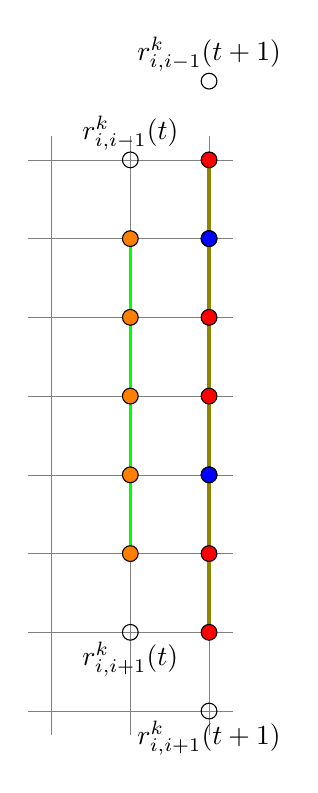
\begin{tikzpicture}[scale=1]
\draw[step=1cm,gray,very thin] (1.7,-4.3) grid (4.3,3.3);
\draw [green,very thick](3,-2)--(3,2);
\draw [olive,very thick](4,-3)--(4,3);
\foreach \y in {-2,...,2}
	{\draw [fill=orange] (3,\y) circle [radius=0.1];}
\foreach \y in {-3,...,3}
	{\draw [fill=red] (3+1,\y) circle [radius=0.1];}
\foreach \y in {-1,2}
	{\draw [fill=blue] (3+1,\y) circle [radius=0.1];}
\draw (3,3) circle [radius=0.1];
\node [above, black] at (3,3) {$r_{i,i-1}^k(t)$};
\draw (3,-3) circle [radius=0.1];
\node [below, black] at (3,-3) {$r_{i,i+1}^k(t)$};
\draw (3+1,3+1) circle [radius=0.1];
\node [above, black] at (3+1,3+1) {$r_{i,i-1}^k(t+1)$};
\draw (3+1,-3-1) circle [radius=0.1];
\node [below, black] at (3+1,-3-1) {$r_{i,i+1}^k(t+1)$};
\end{tikzpicture}

\caption{\label{fig:Fogarty's-dream}Fogarty's dream}
%
\end{minipage}\hfill{}%
\begin{minipage}[t]{0.3\columnwidth}%
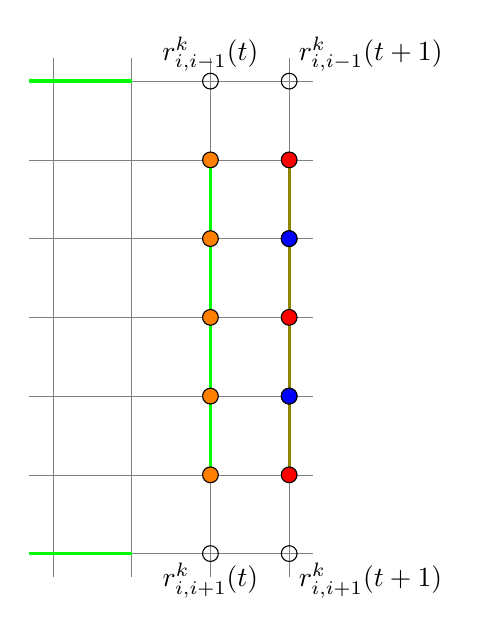
\begin{tikzpicture}[scale=1]
\draw[step=1cm,gray,very thin] (-1.3,-3.3) grid (2.3,3.3);
\draw [green,very thick](1,-2)--(1,2); % L_2 (t)
\draw [olive,very thick](2,-2)--(2,2); % L_2(t+1)
\draw [green,very thick](-1.3,3)--(0,3); % L_1 (t)
\draw [green,very thick](-1.3,-3)--(0,-3); % L_3 (t)
\foreach \y in {-2,...,2}
	{\draw [fill=orange] (1,\y) circle [radius=0.1];}
\foreach \y in {-2,...,2}
	{\draw [fill=red] (2,\y) circle [radius=0.1];}
\foreach \y in {1,-1}
	{\draw [fill=blue] (2,\y) circle [radius=0.1];}
\draw (1,3) circle [radius=0.1];
\node [above, black] at (1,3) {$r_{i,i-1}^k(t)$};
\draw (1,-3) circle [radius=0.1];
\node [below, black] at (1,-3) {$r_{i,i+1}^k(t)$};
\draw (2,3) circle [radius=0.1];
\node [above right, black] at (2,3) {$r_{i,i-1}^k(t+1)$};
\draw (2,-3) circle [radius=0.1];
\node [below right, black] at (2,-3) {$r_{i,i+1}^k(t+1)$};
\end{tikzpicture}

\caption{\label{fig:Corners-are-evil}Corners are evil}
%
\end{minipage}\hfill{}%
\begin{minipage}[t]{0.3\columnwidth}%
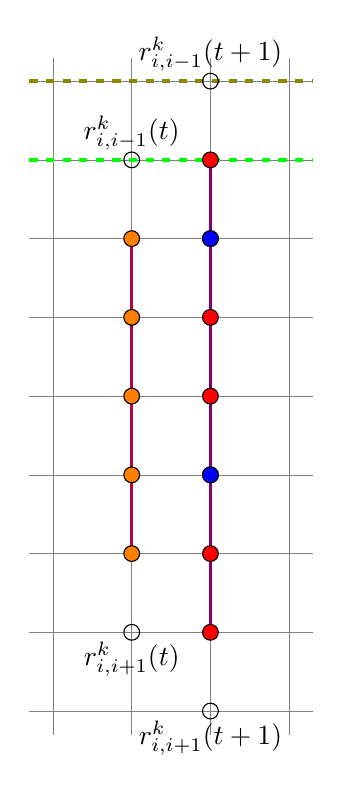
\begin{tikzpicture}[scale=1]
\draw[step=1cm,gray,very thin] (1.7,-4.3) grid (5.3,4.3);
\draw [purple,very thick](3,-2)--(3,2);
\draw [green,dashed, very thick](1.7,3)--(5.3,3);
\draw [olive,very thick,dashed](1.7,4)--(5.3,4);
\draw [violet,very thick](4,-3)--(4,3);
\foreach \y in {-2,...,2}
	{\draw [fill=orange] (3,\y) circle [radius=0.1];}
\foreach \y in {-3,...,3}
	{\draw [fill=red] (3+1,\y) circle [radius=0.1];}
\foreach \y in {-1,2}
	{\draw [fill=blue] (3+1,\y) circle [radius=0.1];}
\draw (3,3) circle [radius=0.1];
\node [above, black] at (3,3) {$r_{i,i-1}^k(t)$};
\draw (3,-3) circle [radius=0.1];
\node [below, black] at (3,-3) {$r_{i,i+1}^k(t)$};
\draw (3+1,3+1) circle [radius=0.1];
\node [above, black] at (3+1,3+1) {$r_{i,i-1}^k(t+1)$};
\draw (3+1,-3-1) circle [radius=0.1];
\node [below, black] at (3+1,-3-1) {$r_{i,i+1}^k(t+1)$};
\end{tikzpicture}

\caption{\label{fig:Y-coordinates}y coordinates}
%
\end{minipage}
\end{figure}

\begin{defn}
Define 
\[
p_{i,j}^{k}\left(t+1\right)=1_{\left(\Phi_{i}^{k}\left(t\right)^{+}\cap L_{j}^{k}\left(t+1\right)\right)}-1_{\left(\Phi_{j}^{k}\left(t\right)^{+}\cap L_{i}^{k}\left(t+1\right)\right)},
\]

and
\[
p_{i}^{k}\left(t+1\right)=p_{i,i+1}^{k}\left(t+1\right)+p_{i,i-1}^{k}\left(t+1\right).
\]
\end{defn}

Which is the quantity to correct the situation.

Observe that $p_{i,j}^{k}$ is anti-symmetric in $i,j$ so that $p_{i,j}^{k}\left(t+1\right)=-p_{j,i}^{k}\left(t+1\right)$.
\begin{cor}
\label{cor:3} Denote by $y_{i}^{k}\left(t\right)$ the y coordinate
of $L_{i}^{k}\left(t\right)$, if $\Delta r_{0}^{k}\left(t\right)=1$
then $y_{0}^{k}\left(t+1\right)=y_{0}^{k}\left(t\right)+1$, notice
that $y_{1}^{k}\left(t\right)<y_{0}^{k}\left(t\right)$ and hence
the y coordinate of $\Phi_{1}^{k}\left(t\right)^{+}$ is smaller from
$y_{0}^{k}\left(t\right)+1$ which obtain $\Phi_{1}^{k}\left(t\right)^{+}\cap L_{0}^{k}\left(t+1\right)=\varnothing$,
use the same argument to deduce $\Phi_{3}^{k}\left(t\right)^{+}\cap L_{0}^{k}\left(t+1\right)=\varnothing$,
conclude:
\[
\Delta r_{i}^{k}\left(t\right)=1\Rightarrow0\leq p_{i\pm1}^{k}\left(t+1\right).
\]

See \figref{Y-coordinates}.

Moreover for all $t$ using anti-symmetric obtains
\[
p^{k}\left(t\right)=\sum_{i\in\left[4\right]}\left(p_{i,i+1}^{k}\left(t\right)+p_{i,i-1}^{k}\left(t\right)\right)=\sum_{i\in\left[4\right]}p_{i,i+1}^{k}\left(t\right)+\sum_{i\in\left[4\right]}p_{i,i-1}^{k}\left(t\right)
\]
\[
=\sum_{i\in\left[4\right]}p_{i,i+1}^{k}\left(t\right)+\sum_{i\in\left[4\right]}p_{i+1,i}^{k}\left(t\right)=0.
\]
\end{cor}

\begin{lem}
\label{lem:2}For all $t$
\begin{equation}
2a_{i}^{k}\left(t\right)+\varphi_{i}^{k}\left(t\right)\leq\varphi_{i}^{k}\left(t+1\right)+f_{i}^{k}\left(t+1\right)+p_{i}^{k}\left(t+1\right).\label{eq:phi_i^j}
\end{equation}
\end{lem}

The lemma will prove at the end of this chapter.
\begin{cor}
Summing (\ref{eq:phi_i^j}) over $\tau=t_{1},...t_{2}-1$ yields 
\[
2\sum_{t_{1}}^{t_{2}-1}a_{i}^{k}\left(\tau\right)+\sum_{t_{1}}^{t_{2}-1}\varphi_{i}^{k}\left(\tau\right)\leq\sum_{t_{1}+1}^{t_{2}}\varphi_{i}^{k}\left(\tau\right)+\sum_{t_{1}+1}^{t_{2}}f_{i}^{k}\left(\tau\right)+\sum_{t_{1}+1}^{t_{2}}p_{i}^{k}\left(\tau\right),
\]

omit $2\sum_{t_{1}}^{t_{2}-1}a_{i}^{k}\left(\tau\right)$ from the
LHS to obtain
\[
\varphi_{i}^{k}\left(t_{1}\right)-\sum_{t_{1}+1}^{t_{2}}f_{i}^{k}\left(\tau\right)-\sum_{t_{1}+1}^{t_{2}}p_{i}^{k}\left(\tau\right)\leq\varphi_{i}^{k}\left(t_{2}\right).
\]
\end{cor}

Lastly provide lower bound to $p_{i}$ (the only negative quantity
in this paper).
\begin{lem}
\label{lem:3}For all $t\in\mathbb{N}$ we have:
\[
\varphi_{i}\left(0\right)-6h^{4}\leq f_{i}\left(t\right)^{\ast}+p_{i}\left(t\right)^{\ast}.
\]
\end{lem}

\begin{proof}
Let $t\in\mathbb{N}$ , and for all $k$ denote $t_{i}^{k}=\max_{\tau<t}\Delta r_{i}^{k}\left(\tau\right)=0$.

Summation on \ref{eq:phi_i^j} from 0 to $t_{i}^{k}$ yields 
\[
\varphi_{i}^{k}\left(0\right)+2a_{i}^{k}\left(t_{i}^{k}\right)^{\ast}\leq\varphi_{i}^{k}\left(t_{i}^{k}\right)+f_{i}^{k}\left(t_{i}^{k}\right)^{\ast}+p_{i}^{k}\left(t_{i}^{k}\right)^{\ast},
\]

$\Delta r_{i}^{k}\left(t_{i}^{k}\right)=0$ so that $\varphi_{i}^{k}\left(t_{i}^{k}\right)<\alpha_{i}^{k}\left(t_{i}^{k}\right)$
and
\[
\varphi_{i}^{k}\left(0\right)+2a_{i}^{k}\left(t_{i}^{k}\right)^{\ast}\leq\alpha_{i}^{k}\left(t_{i}^{k}\right)+f_{i}^{k}\left(t_{i}^{k}\right)^{\ast}+p_{i}^{k}\left(t_{i}^{k}\right)^{\ast}.
\]
Maximality of $t_{i}^{k}$ and \corref{3} guarantees $0\leq p_{i}^{k}\left(\tau\right)$
for all $t_{i}^{k}\leq\tau$, use $0\leq\sum_{t_{i}^{k}+1}^{t}p_{i}^{k}\left(\tau\right),0\leq\sum_{t_{i}^{k}+1}^{t}f_{i}^{k}\left(\tau\right)$
to obtain
\[
\varphi_{i}^{k}\left(0\right)+2a_{i}^{k}\left(t_{i}^{k}\right)^{\ast}\leq\alpha_{i}^{k}\left(t_{i}^{k}\right)+f_{i}^{k}\left(t\right)^{\ast}+p_{i}^{k}\left(t\right)^{\ast},
\]
summing on $k$ and omitting $2a_{i}^{k}\left(t_{i}^{k}\right)^{\ast}$
from the LHS yields
\[
\varphi_{i}\left(0\right)-h\max_{\tau<t,i\in\left[4\right],k\in\left[h\right]}\left(\alpha_{i}^{k}\left(\tau\right)\right)\leq f_{i}\left(t\right)^{\ast}+p_{i}\left(t\right)^{\ast},
\]
use $\alpha_{i}^{k}\left(t\right)\leq6h^{3}$ to conclude
\[
\varphi_{i}\left(0\right)-6h^{4}\leq f_{i}\left(t\right)^{\ast}+p_{i}\left(t\right)^{\ast}.
\]
\end{proof}

\section{Fire overflow and pulls}

Toward proving (\ref{lem:2}) we want to bound the potential from
above, the potential contains in the correspond front and hence bound
by the front length, an easy observation shows that 
\[
\left|L_{i}^{k}\left(t\right)\right|=r_{\left\{ i-1,i+1\right\} }^{k}\left(t\right)
\]
and hence we want to bound the quantity of pulls. This section define
another quantity of fire, in addition to the potential and use this
quantity to dominate the quantity of pulls
\begin{defn}
According to \lemref{2} define the $overflow$ of the k-level i-th
front which denoted by $o_{i}^{k}\left(t\right)$, to be the positive
number that satisfies the equation:
\begin{equation}
2a_{i}^{k}\left(t\right)+\varphi_{i}^{k}\left(t\right)+o_{i}^{k}\left(t\right)=\varphi_{i}^{k}\left(t+1\right)+f_{i}^{k}\left(t+1\right)+p_{i}^{k}\left(t+1\right).\label{eq:i j}
\end{equation}
\end{defn}

\begin{cor}
Summation (\ref{eq:i j}) over $i\in\left[4\right],k\in\left[h\right],\tau\in\left[1,t-1\right]$
yields:
\[
2a\left(t\right)^{\ast}+\varphi\left(0\right)+o\left(t\right)^{\ast}=\varphi\left(t\right)+f\left(t\right)+p\left(t+1\right)^{\ast}.
\]

using $p\left(t\right)^{\ast}=0$ gives
\begin{equation}
\varphi\left(0\right)+2a\left(t\right)^{\ast}+o\left(t\right)^{\ast}=\varphi\left(t\right)+f\left(t\right).\label{eq:*}
\end{equation}
\end{cor}

\begin{lem}
\label{lem:4} for all $t\in\mathbb{N}$ if there is a pulled level
in the i-th front then
\[
\begin{cases}
2h<o_{i}\left(t\right) & g_{i}\left(t\right)=1\\
6h^{2}<o_{i}\left(t\right) & g_{i}\left(t\right)=0
\end{cases}.
\]
\end{lem}

\begin{proof}
For all $k$, denote $\Phi_{i}^{k}\left(t\right)=L_{i}^{k}\left(t\right)\cap B_{i}^{k}\left(t\right)$
which are the sets of the the i-th k-th fire. Let k such that the
k-th level being pulled by the $\ell$-th level and take $\ell$ to be minimal. Using \claimautorefname{}
by \corref{4} we have $r_{i}^{\ell-1}\left(t\right)=r_{i}^{\ell}\left(t\right)-1$
therefore fire $\Phi_{i}^{\ell}\left(t\right)$ adjacent to $L_{i}^{\ell-1}\left(t+1\right)$
and therefore
\[
\varphi_{i}^{\ell}\left(t\right)-2\leq\varphi_{i}^{\ell-1}\left(t+1\right)+f_{i}^{\ell-1}\left(t+1\right)
\]
(the addition of $-2$ is due to the corners). The $\ell$-th level
is spreading, therefore $\alpha_{i}^{\ell}\left(t\right)<\left|\Phi_{i}^{\ell}\left(t\right)\right|$.
Minimality of $\ell$ gives that the $\ell-1$-th level not pulling
the k-th level, that $a_{i}^{\ell-1}\left(t\right)=0$ and hence $\left|\Phi_{i}^{\ell-1}\left(t\right)\right|\leq\alpha_{i}^{\ell-1}\left(t\right)$.
Deduce
\[
\alpha_{i}^{\ell}\left(t\right)-\alpha_{i}^{\ell-1}\left(t\right)<\varphi_{i}^{\ell}\left(t\right)-\varphi_{i}^{\ell-1}\left(t\right),
\]
together with $-1\leq p_{i}^{\ell}\left(t+1\right)$ and the definition
of $o_{i}^{\ell}\left(t\right)$, conclude: 
\[
\varphi_{i}^{\ell-1}\left(t+1\right)+f_{i}^{\ell-1}\left(t+1\right)+p_{i}^{\ell-1}\left(t+1\right)-\left(\varphi_{i}^{\ell-1}\left(t\right)+2a_{i}^{\ell-1}\left(t\right)\right)=o_{i}^{\ell-1}\left(t\right)
\]
\[
\left(\varphi_{i}^{\ell}\left(t\right)-2\right)-2-\left(\varphi_{i}^{\ell-1}\left(t\right)\right)\leq,
\]

conclude
\[
\alpha_{i}^{\ell}\left(t\right)-\alpha_{i}^{\ell-1}\left(t\right)-4\leq o_{i}^{\ell-1}\left(t\right).
\]

Now, $g_{i}\left(t\right)=1$ yields
\[
2h+2=\left(2h+2\right)\left(\left(r_{i}^{\ell}\left(t\right)-r_{i}^{\min}\left(t\right)+1\right)-\left(r_{i}^{\ell-1}\left(t\right)-r_{i}^{\min}\left(t\right)+1\right)\right)=\alpha_{i}^{\ell}\left(t\right)-\alpha_{i}^{\ell-1}\left(t\right),
\]
and $g_{i}\left(t\right)=0$ yields
\[
6h^{2}+2=\left(6h^{2}+2\right)\left(\left(r_{i}^{\ell}\left(t\right)-r_{i}^{\min}\left(t\right)+1\right)-\left(r_{i}^{\ell-1}\left(t\right)-r_{i}^{\min}\left(t\right)+1\right)\right)=\alpha_{i}^{\ell}\left(t\right)-\alpha_{i}^{\ell-1}\left(t\right).
\]
\end{proof}
\begin{cor}
\label{cor:6} Let $t\in\mathbb{N}$ if there is a pull in the i-th
front then at most $h-1$ of the levels are pulled, then the quantity
of the pull is less then $h-1$ and hence 
\[
\Delta r_{i}\left(t\right)\leq a_{i}\left(t\right)+\left(h-1\right)\leq a_{i}\left(t\right)+\frac{1}{2}o_{i}\left(t\right).
\]
Use the observation at the beginning of this section to conclude:
\begin{align}
\varphi_{i}\left(t\right)\leq\sum_{k\in\left[h\right]}\left|L_{i}^{k}\left(t\right)\right|=r_{\left\{ i-1,i+1\right\} }\left(t\right) & =r_{\left\{ i-1,i+1\right\} }\left(1\right)+\sum_{0}^{t}\Delta r_{\left\{ i-1,i+1\right\} }\left(\tau\right)\nonumber \\
 & \leq r_{\left\{ i-1,i+1\right\} }\left(1\right)+a_{\left\{ i-1,i+1\right\} }\left(t\right)^{\ast}+\frac{1}{2}o_{\left\{ i-1,i+1\right\} }\left(t\right)^{\ast}.\label{eq:rho upper}
\end{align}
\end{cor}


\section{Paying the debt}

In this section we define the global spreading, which is ``almost''
the sum of the local spreading. Our goal is to quantitate this ``almost''
and bound it from above by the overflow.
\begin{defn}
Define $b_{i}\left(t\right)=\max_{k\in\left[h\right]}\left(a_{i}^{k}\left(t\right)\right)$
and denote the $debt$ of the i-th front by: 
\[
s_{i}\left(t\right)=hb_{i}\left(t\right)-a_{i}\left(t\right).
\]
\end{defn}

Note that in the symmetric toy model all the levels are spread or
simultaneously therefore $s_{i}\left(t\right)=0$ for all $t$, using
\cite{FH} one can deduce that in this model 
\[
3h\leq hb_{i}\left(t\right)=a_{i}\left(t\right).
\]
Think of the debt as quantitating how much the situation different
from the symmetric model.
\begin{defn}
Denote $q\left(t\right):=b\left(t\right)-3$, which indicate if there
are four spreading front.
\end{defn}

The following proposition shows us that the situation is close to
the symmetric model.
\begin{prop}
\label{prop:debt bound}For all $t$ the following inequality holds
\[
s\left(t\right)^{\ast}\leq\frac{1}{2}o\left(t\right)^{\ast}+hq\left(t\right)^{\ast}+8h^{2}.
\]
\end{prop}

The proof appear after the next two definitions
\begin{defn}
The i-th front is $Getting\,blocked$ (from time $t$ to $w$) if
there is a sequence $t\leq t_{i}^{k}\leq w$ such that $a_{i}^{k}\left(t_{i}^{k}\right)=0$.

Denote by $\beta_{i}\left(t\right)$ the amount of time the i-th front
spend getting blocked.
\end{defn}

\begin{rem*}
May be there are more then one blocking sequence in this case take
the one with the minimal $w$.
\end{rem*}
Getting blocked generalize the idea of $a_{i}\left(t\right)=0$.

This section shows that $\beta_{i}\left(t\right)$ is a local version
of $q\left(t\right)$ and hence 
\[
s\left(t\right)^{\ast}\leq\frac{1}{2}o\left(t\right)^{\ast}+h\beta_{i}\left(t\right)+2h^{2},
\]
is the local version of (\ref{prop:debt bound}) ,with this intuition
come this definition of $g_{i}\left(t\right)$.
\begin{defn}
Define the indicator of ``paying the debt'' in the i-th front
\[
g_{i}\left(t\right)=\begin{cases}
1 & s\left(t\right)^{\ast}\leq\frac{1}{2}o\left(t\right)^{\ast}+h\beta_{i}\left(t\right)\\
0 & \text{otherwise}
\end{cases}.
\]
\end{defn}

\begin{proof}
First show that high debt cause a interesting event.
\begin{lem}
\label{lem:5} Let $t$ with $g_{i}\left(t-1\right)=1,g_{i}\left(t\right)=0$
then there is $w\in\left(t,t+2h\right)$ and one of the following:
\begin{enumerate}
\item $Reactivate$ - there is $k$ with $a_{i}^{k}\left(w\right)=1,a_{i}^{k}\left(t\right)=0$.
\item There is a pulled level at time $w$ in the i-th front.
\item The i-th front is Getting blocked from time $t$ to $w$.
\end{enumerate}
\end{lem}

\begin{proof}
Observe that $g_{i}\left(t-1\right)=1,g_{i}\left(t\right)=0$ implies
that $s_{i}\left(t\right)>0$ and hence there is $\ell$ with $a_{i}^{\ell}\left(t\right)=0$,
so that $\varphi_{i}^{\ell}\left(t\right)<\alpha_{i}^{\ell}\left(t\right)$,
use $1=g_{i}\left(t-1\right)$ to obtain $\varphi_{i}^{\ell}\left(t\right)\leq2h^{2}$.
Now separate to different cases.

Case 1: there is $w$ with $a_{i}^{\ell}\left(w\right)=1$ and hence
$\alpha_{i}^{\ell}\left(w\right)<\varphi_{i}^{\ell}\left(w\right)$,
therefore
\[
\left(2h-2\right)h=\frac{4h^{2}-4h}{2}\leq\frac{\alpha_{i}^{\ell}\left(w\right)-\alpha_{i}^{\ell}\left(t\right)-4h}{2}\leq\frac{\varphi_{i}^{\ell}\left(w\right)-\varphi_{i}^{\ell}\left(t\right)-\sum_{t}^{w-1}p_{i}^{\ell}\left(\tau\right)}{2}\leq\frac{1}{2}\sum_{t}^{w-1}o_{i}^{\ell}\left(\tau\right).
\]

Case 2: First assume that $a_{i}^{\ell}\left(\tau\right)=0$ for all
$\tau\in\left(t,t+2h-2\right)$, observe that $\Delta r_{i}^{\ell}\left(\tau\right)=1$
implies pull and hence assume $\Delta r_{i}^{\ell}\left(\tau\right)=0$.
If there is $m$ with $a_{i}^{m}\left(\tau\right)=1$ for all $\tau\in\left(t,t+2h-2\right)$
then
\[
h-1\leq2h-2-\left(h-1\right)\leq2h-2+r_{i}^{m}\left(t\right)-r_{i}^{\ell}\left(t\right)=r_{i}^{m}\left(t+2h-2\right)-r_{i}^{\ell}\left(t+2h-2\right)
\]
and hence all the levels between $\ell$ and $m$ are getting pulled
at some $w\in\left(t,t+2h-2\right)$. By \lemref{4} and the fact
that $g_{i}\left(w\right)=0$ we have 
\[
2h^{2}\leq o_{i}^{m}\left(w\right).
\]

Case 3: For all $k$ there is $\tau^{k}\in\left(t,t+2h-2\right)$
with $a_{i}^{k}\left(\tau^{k}\right)=0$.

Use the trivial bound $s_{i}\left(\tau\right)\leq h-1$ to conclude
that 
\[
\sum_{t}^{w}s_{i}\left(\tau\right)\leq\sum_{t}^{w}o_{i}\left(\tau\right)+h\left(\beta_{i}\left(w\right)-\beta_{i}\left(t\right)\right).
\]
\end{proof}

\begin{cor}
Combine the last inequity with the fact that $g_{i}\left(t-1\right)=1$
to obtain
\[
s_{i}\left(w\right)^{\ast}\leq o_{i}\left(w\right)^{\ast}+h\beta_{i}\left(w\right),
\]
conclude that for all $t$ such that $g_{i}\left(t-1\right)=1,g_{i}\left(t\right)=0$
we have $t<w<t+2h$ with $g_{i}\left(w\right)=1$. 
\end{cor}

\begin{cor}
Let $t$ with $g_{i}\left(t\right)=0$ take maximal $\tau$ with $g_{i}\left(\tau\right)=1$
and $\tau\leq t$. The last corollary arise $\tau<w\leq\tau+2h$ with
$g_{i}\left(w\right)=1$, if $\tau\leq t-2h$ then $w$ contradicts
the maximality of $\tau$. conclude that
\[
s_{i}\left(t\right)^{\ast}\leq s_{i}\left(\tau\right)^{\ast}+2h^{2}\leq o_{i}\left(\tau\right)^{\ast}+\beta_{i}\left(\tau\right)+2h^{2}\leq o_{i}\left(t\right)^{\ast}+\beta_{i}\left(t\right)+2h^{2},
\]
when the first inequity uses $t\leq\tau+2h$ and $s_{i}\left(u\right)\leq h-1$,
the second uses $g_{i}\left(\tau\right)=1$ and the third by non negativity
of $o_{i}\left(u\right),\Delta\beta_{i}\left(u\right)$.
\end{cor}

\begin{lem}
No two front are getting blocked simultaneously and while front is
getting blocked we have $q\left(\tau\right)=1$
\end{lem}

\begin{proof}
Assume by contradiction that there are two sequences $t_{i}\leq t_{i}^{k}\leq w_{i},t_{j}\leq t_{j}^{k}\leq w_{j}$
such that $a_{j}^{k}\left(t_{j}^{k}\right)=a_{i}^{k}\left(t_{i}^{k}\right)=0$
and $\left[t_{i},w_{i}\right]\cap\left[t_{j},w_{j}\right]\ne\varnothing$,
use to non trivial intersection and $w_{i}-t_{i}<2h,w_{j}-t_{j}<2h$
to obtain that the length of $\left[t_{i},w_{j}\right]$ is less then
$4h$ (we assuming $t_{i}\leq t_{j}$) and deduce $t_{j}^{k}\in\left[t_{i},t_{i}+4h\right]$,
use \lemref{1} to obtain 
\[
12h^{4}\leq\sum_{k\in\left[h\right]}\varphi_{i}^{k}\left(t_{i}^{k}\right)+\varphi_{j}^{k}\left(t_{j}^{k}\right)=0,
\]
by contradiction.

By definition $b_{i}\left(t\right)$ is the maximum over $a_{i}^{k}\left(t\right)$
therefore it suffice to find spreading level on each front. Let $t_{i}\leq\tau\leq w_{i}$
, put $t_{j}=t_{i},w_{j}=w_{i}$ and $t_{j}^{k}=\tau$ use \lemref{1}
again to obtain $12h^{4}\leq\sum_{k\in\left[h\right]}\varphi_{j}^{k}\left(\tau\right)=\varphi_{j}\left(\tau\right)$,
by pigeonhole principal there is $m\in\left[h\right]$ with $\alpha_{j}^{m}\left(t\right)\leq6h^{3}\leq\varphi_{j}^{m}\left(\tau\right)$
and hence the j-th front has active level. The minimality of $w$
guarantee that $0<a_{i}\left(\tau\right)$ for all $t_{i}\leq\tau<w_{i}$
and hence all four fronts have have active level during the blocking
processes. 
\end{proof}
\begin{cor}
Use the previews lemma to obtain
\[
\sum_{i\in\left[4\right]}\beta_{i}\left(t\right)\leq\sum_{\tau\leq t}q\left(\tau\right)=q\left(t\right)^{\ast}.
\]

and the last corollary to conclude
\[
s\left(t\right)^{\ast}=\sum_{i\in\left[4\right]}s_{i}\left(t\right)^{\ast}\leq\sum_{i\in\left[4\right]}\left(o_{i}\left(t\right)^{\ast}+h\beta_{i}\left(t\right)+2h^{2}\right)\leq o\left(t\right)^{\ast}+hq\left(t\right)^{\ast}+8h^{2}.
\]
\end{cor}

\end{proof}
\begin{cor}
\label{cor:5}Combine the definitions of $a,b,q$ and $s$ with the
previews corollary and get
\[
3ht+\frac{1}{2}o\left(t\right)^{\ast}-8h^{2}\leq hq\left(t\right)^{\ast}+3ht-s^{\ast}\left(t\right)+o\left(t\right)^{\ast}=a\left(t\right)^{\ast}+o\left(t\right)^{\ast}.
\]
\end{cor}


\section{Proof of \lemref{1}}

This section will shows the proof of \lemref{1} and the details of
\lemref{2} proof.
\begin{proof}
Let $k\in\left[h\right],i,j\in\left[4\right]$ and $i\ne j$, let
$0\leq\delta_{i}^{k},\delta_{j}^{k}<4h$. For all $t\in\mathbb{N}$
denote: $A_{i,j}\left(t\right)=\sum_{k\in\left[h\right]}\varphi_{i}^{k}\left(t+\delta_{i}^{k}\right)+\varphi_{j}^{k}\left(t+\delta_{j}^{k}\right)$.

From \lemref{2} we have that 
\[
\varphi_{i}^{k}\left(t\right)-\sum_{w=t+1}^{t+\delta_{i}^{k}}\left(f_{i}^{k}\left(\tau\right)+p_{i}^{k}\left(\tau\right)\right)\leq\varphi_{i}^{k}\left(t+\delta_{i}^{\beta}\right),
\]
therefore
\[
\sum_{k\in\left[h\right]}\left(\varphi_{i}^{k}\left(t\right)-\delta_{i}^{k}-\sum_{w=t}^{t+\delta_{i}^{k}-1}f_{i}^{k}\left(w\right)\right)+\sum_{k\in\left[h\right]}\left(\varphi_{j}^{k}\left(t\right)-\delta_{j}^{k}-\sum_{w=t}^{t+\delta_{j}^{k}-1}f_{j}^{k}\left(w\right)\right)\leq\sum_{k\in\left[h\right]}\varphi_{i}^{k}\left(t+\delta_{i}^{k}\right)+\sum_{k=1}^{h}\varphi_{j}^{k}\left(t+\delta_{j}^{k}\right),
\]
use $\delta_{i}^{k},\delta_{j}^{k}\leq4h$ 
\[
\sum_{k\in\left[h\right]}\left(\varphi_{i}^{k}\left(t\right)-4h-\sum_{w=t}^{t+\delta_{i}^{k}-1}f_{i}^{k}\left(w\right)\right)+\sum_{k\in\left[h\right]}\left(\varphi_{j}^{k}\left(t\right)-4h-\sum_{w=t}^{t+\delta_{j}^{k}-1}f_{j}^{k}\left(w\right)\right)\leq
\]
and $0\leq f_{i}^{k}\left(w\right)$ yields 
\[
\sum_{k\in\left[h\right]}\left(\varphi_{i}^{k}\left(t\right)-4h-\sum_{w=t}^{t+4h}f_{i}^{k}\left(w\right)\right)+\sum_{k\in\left[h\right]}\left(\varphi_{j}^{k}\left(t\right)-4h-\sum_{w=t}^{t+4h}f_{j}^{k}\left(w\right)\right)\leq
\]
\begin{equation}
\varphi_{ij}\left(t\right)-8h^{2}-\sum_{w=t}^{t+4h}f_{\left\{ i,j\right\} }\left(w\right)=.\label{eq:1}
\end{equation}

Take the initial fire $S\subseteq\mathbb{Z}\boxtimes\mathbb{Z}\times\left[h\right]$
to be the box 
\[
\left[-6h^{3}-1,6h^{3}+1\right]\times\left[h\right]
\]
and choose $r_{i}^{k}\left(0\right)=6h^{3}$, which yields 
\[
2r_{02}\left(0\right)=r\left(0\right)=\sum_{i\in\left[4\right]}\sum_{k\in\left[h\right]}r_{i}^{k}\left(0\right)=24h^{4},
\]
 and 
\[
2\varphi_{\left\{ i,j\right\} }\left(0\right)=\varphi\left(0\right)=\sum_{i\in\left[4\right]}\sum_{k\in\left[h\right]}\left(2r_{i}^{k}\left(0\right)-1\right)=2r\left(0\right)-4h=48h^{4}-4h.
\]
Use (\ref{eq:1}) with $t=0$ gives 
\[
\varphi_{ij}\left(0\right)-8h^{2}-\sum_{w=0}^{4h}f_{\left\{ i,j\right\} }\left(w\right)\leq A
\]
and $f_{ij}\left(t\right)^{\ast}\leq f\left(t\right)^{\ast}\leq3ht$
gives 
\[
48h^{4}-7h-20h^{2}=48h^{4}-4h-8h^{2}-3h-12h^{2}\leq\varphi_{ij}\left(1\right)-8h^{2}-3h-12h^{2}\leq A,
\]
conclude that 
\[
12h^{4}\leq A_{i,j}\left(0\right).
\]

Inductively assume \lemref{1} holds for all $\tau<t$ and hence all
the previews results holds. From \corref{3<b} we know that $3\leq b\left(\tau\right)$
so $3t\leq b\left(t\right)^{\ast}$.

Assume the i-th front is adjacent to the j-th front and for brevity
put $i=0,j=1$.

Use (\ref{eq:rho upper}) on the third and forth fronts to obtain
\[
\varphi_{\left\{ 2,3\right\} }\left(t\right)\leq r\left(1\right)+a\left(t\right)^{\ast}+\frac{1}{2}o\left(t\right)^{\ast},
\]

combine with (\ref{eq:1}) and get
\[
\left(\varphi_{\left\{ 0,1\right\} }\left(t\right)-8h^{2}-\sum_{w=t}^{t+4h}f_{\left\{ 0,1\right\} }\left(w\right)\right)+\left(\varphi_{\left\{ 2,3\right\} }\left(t\right)-\left(r\left(1\right)+a\left(t\right)^{\ast}+\frac{1}{2}o\left(t\right)^{\ast}\right)\right)\leq
\]
\begin{equation}
\varphi\left(t\right)-8h^{2}-\sum_{w=t}^{t+4h}f_{\left\{ 0,1\right\} }\left(w\right)-r\left(1\right)-a\left(t\right)^{\ast}-\frac{1}{2}o\left(t\right)^{\ast}=\label{eq:2}
\end{equation}
Stop for a moment to calculate a lower bound for $\varphi\left(t\right)-\sum_{w=t}^{t+4h-1}f_{\left\{ 0,1\right\} }\left(w\right)$.

Subtract $\sum_{w=t}^{t+4h-1}f_{\left\{ 0,1\right\} }\left(w\right)$
from (\ref{eq:*}) to get:
\[
2a\left(t\right)^{\ast}+\varphi\left(1\right)+o\left(t\right)^{\ast}-f\left(t\right)^{\ast}-\sum_{w=t}^{t+4h-1}f_{\left\{ 0,1\right\} }\left(w\right)=\varphi\left(t\right)-\sum_{w=t}^{t+4h-1}f_{\left\{ 0,1\right\} }\left(w\right),
\]
by $f_{\left\{ 0,1\right\} }\left(w\right)\leq f\left(w\right)$
\[
\varphi\left(1\right)+2a\left(t\right)^{\ast}+o\left(t\right)^{\ast}-f\left(t+4h\right)^{\ast}\leq\varphi\left(t\right)-\sum_{w=t}^{t+4h-1}f_{\left\{ 0,1\right\} }\left(w\right),
\]

by $f\left(t\right)^{\ast}\leq3ht$
\[
\varphi\left(1\right)+2a\left(t\right)^{\ast}+o\left(t\right)^{\ast}-3ht-12h^{2}\leq\varphi\left(t\right)-\sum_{w=t}^{t+4h-1}f_{\left\{ 0,1\right\} }\left(w\right).
\]

By \corref{5} $3ht-8h^{2}\leq a\left(t\right)^{\ast}+\frac{1}{2}o\left(t\right)^{\ast}$
and hence 
\[
\varphi\left(1\right)+3ht+\frac{1}{2}o\left(t\right)^{\ast}-8h^{2}+a\left(t\right)^{\ast}-3ht-12h^{2}\leq\varphi\left(t\right)-\sum_{w=t}^{t+4h-1}f_{\left\{ 0,1\right\} }\left(w\right)
\]
\begin{equation}
\varphi\left(1\right)+a\left(t\right)^{\ast}+\frac{1}{2}o\left(t\right)^{\ast}-20h^{2}\leq\varphi\left(t\right)-\sum_{w=t}^{t+4h-1}f_{\left\{ 0,1\right\} }\left(w\right).\label{eq:3}
\end{equation}
\begin{rem*}
For opposite fronts, use the same arguments ((\ref{eq:*}) and \corref{5})
and get following inequality 
\begin{equation}
\varphi\left(1\right)+6ht-16h^{2}-f\left(t\right)^{\ast}\leq\varphi\left(t\right).\label{eq:5}
\end{equation}
\end{rem*}
combine (\ref{eq:2}) and (\ref{eq:3})
\[
\varphi\left(1\right)+a\left(t\right)^{\ast}+\frac{1}{2}o\left(t\right)^{\ast}-20h^{2}-8h^{2}-r\left(1\right)-a\left(t\right)^{\ast}-\frac{1}{2}o\left(t\right)^{\ast}\leq
\]
\[
r\left(1\right)-4h-28h^{2}=\varphi\left(1\right)-28h^{2}-r\left(1\right)=,
\]
use $r\left(1\right)$ calculation to obtain
\[
24h^{4}-4h-28h^{2}\leq A_{ij}\left(t\right)
\]
 and conclude that for all for all $h\geq2$ we have
\[
12h^{4}\leq A_{ij}\left(t\right)=\sum_{k\in\left[h\right]}\varphi_{i}^{k}\left(t+\delta_{i}^{k}\right)+\varphi_{j}^{k}\left(t+\delta_{j}^{k}\right).
\]

Assume the i-th front is opposite to the j-th front and put $i=1,j=3$.
Take (\ref{eq:1}) and multiple it by 2 to get
\[
2\varphi_{\left\{ 0,2\right\} }\left(t\right)-16h^{2}-2\sum_{w=t}^{t+4h-1}f_{\left\{ 0,2\right\} }\left(w\right)\leq2A_{i,j}\left(t\right).
\]

Use (\ref{eq:rho upper}) to obtain 
\[
2\varphi_{\left\{ 0,2\right\} }\left(t\right)-16h^{2}-2\sum_{w=t}^{t+4h-1}f_{\left\{ 0,2\right\} }\left(w\right)+\varphi_{\left\{ 1,3\right\} }-\left(2r_{\left\{ 0,2\right\} }\left(0\right)+2a_{\left\{ 0,2\right\} }\left(t\right)^{\ast}+2o_{\left\{ 0,2\right\} }\left(t\right)^{\ast}\right)\leq
\]
\begin{equation}
\varphi\left(t\right)+\varphi_{\left\{ 0,2\right\} }\left(t\right)-16h^{2}-2\sum_{w=t}^{t+4h-1}f_{\left\{ 0,2\right\} }\left(w\right)-2r_{\left\{ 0,2\right\} }\left(0\right)-2a_{\left\{ 0,2\right\} }\left(t\right)^{\ast}-2o_{\left\{ 0,2\right\} }\left(t\right)^{\ast}=.\label{eq:4}
\end{equation}
Stop for a moment to bound $a_{\left\{ 0,2\right\} }\left(t\right)$
from above:

First, by (\ref{eq:i j})
\[
\varphi_{\left\{ 0,2\right\} }\left(0\right)+2a_{\left\{ 0,2\right\} }\left(t\right)^{\ast}+o_{\left\{ 0,2\right\} }\left(t\right)^{\ast}=\varphi_{\left\{ 0,2\right\} }\left(t\right)+f_{\left\{ 0,2\right\} }\left(t\right)^{\ast}+p_{\left\{ 0,2\right\} }\left(t\right)^{\ast},
\]
\lemref{3} provides $\varphi_{\left\{ 1,3\right\} }\left(0\right)-8h^{4}\leq f_{\left\{ 1,3\right\} }\left(t\right)^{\ast}+p_{\left\{ 1,3\right\} }\left(t\right)^{\ast}$,
together with the last equality we see that:
\[
\varphi\left(0\right)+o_{\left\{ 0,2\right\} }\left(t\right)^{\ast}-8h^{4}-\varphi_{\left\{ 0,2\right\} }\left(t\right)-f\left(t\right)^{\ast}\leq-2a_{\left\{ 0,2\right\} }\left(t\right)^{\ast}.
\]
Combine the last inequality with (\ref{eq:4}) to get 
\[
\varphi\left(t\right)+\varphi_{\left\{ 0,2\right\} }\left(t\right)-16h^{2}-2\sum_{w=t}^{t+4h-1}f_{\left\{ 0,2\right\} }\left(w\right)-2r_{\left\{ 0,2\right\} }\left(0\right)+\left(\varphi\left(0\right)+o_{\left\{ 0,2\right\} }\left(t\right)^{\ast}-8h^{4}-\varphi_{\left\{ 0,2\right\} }\left(t\right)-f\left(t\right)^{\ast}\right)-2o_{\left\{ 0,2\right\} }\left(t\right)^{\ast}\leq
\]
\[
\varphi\left(0\right)-2r_{\left\{ 0,2\right\} }\left(0\right)-16h^{2}-8h^{4}+\varphi\left(t\right)-2\sum_{w=t}^{t+4h-1}f_{\left\{ 0,2\right\} }\left(w\right)-f\left(t\right)^{\ast}=,
\]

now use the remark (\ref{eq:5})  to get 
\[
\varphi\left(0\right)-2r_{\left\{ 0,2\right\} }\left(0\right)-16h^{2}-8h^{4}+\varphi\left(0\right)+6ht-16h^{2}-f\left(t\right)^{\ast}-2\sum_{w=t}^{t+4h-1}f_{\left\{ 0,2\right\} }\left(w\right)-f\left(t\right)^{\ast}\leq
\]
\[
2\varphi\left(0\right)-2r_{\left\{ 0,2\right\} }\left(0\right)-8h^{4}-32h^{4}+6ht-2\left(\sum_{w=t}^{t+4h-1}f_{\left\{ 0,2\right\} }\left(w\right)+f\left(t\right)^{\ast}\right)=,
\]
 using $f\left(t\right)^{\ast}\leq3ht$ yields 
\[
2\varphi\left(0\right)-2r_{\left\{ 0,2\right\} }\left(0\right)-8h^{4}-32h^{4}+6ht-6ht-24h^{2}\leq
\]
\[
2\varphi\left(0\right)-2r_{\left\{ 0,2\right\} }\left(0\right)-56h^{2}-8h^{4}=,
\]
therefore
\[
\varphi\left(0\right)-r_{\left\{ 0,2\right\} }\left(0\right)-28h^{2}-4h^{4}\leq A_{i,j}\left(t\right).
\]
Use $\varphi\left(0\right),r_{\left\{ i,j\right\} }\left(0\right)$
calculations to obtain
\[
48h^{4}-4h-12h^{4}-28h^{2}-4h^{4}\leq A_{i,j}\left(t\right)
\]
 and conclude that for all for all $h\geq2$ we have
\[
12h^{4}\leq A_{i,j}\left(t\right)=\sum_{k=1}^{h}\varphi_{i}^{k}\left(t+\delta_{i}^{k}\right)+\varphi_{j}^{k}\left(t+\delta_{j}^{k}\right).
\]
\end{proof}

\paragraph{proof of Fogarty}

our goal is to proof that
\[
2a_{i}^{k}\left(t\right)+\varphi_{i}^{k}\left(t\right)\leq\varphi_{i}^{k}\left(t+1\right)+f_{i}^{k}\left(t+1\right)+p_{i}^{k}\left(t+1\right).
\]

Remind that $p_{i,j}^{k}\left(t+1\right)=1_{\left|\Phi_{i}^{k}\left(t\right)^{+}\cap L_{j}^{k}\left(t+1\right)\right|=0}-1_{\left|\Phi_{j}^{k}\left(t\right)^{+}\cap L_{i}^{k}\left(t+1\right)\right|=0}$.
\begin{proof}
Look at the corner of the first and second fronts (at the k-th level)

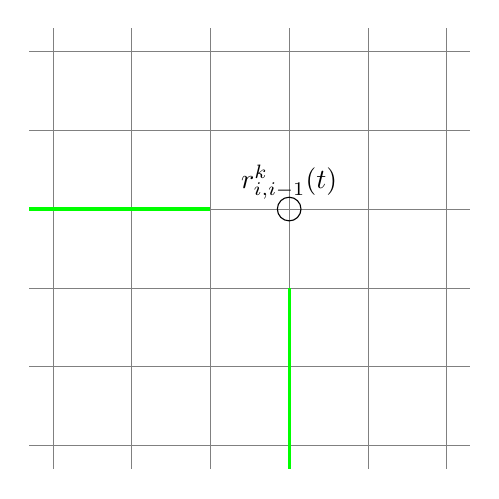
\begin{tikzpicture}[scale=1]
\draw[step=1cm,gray,very thin] (-0.3,-0.3) grid (5.3,5.3);
\draw [green, very thick](-0.3,3)--(2,3);
\draw [green,very thick](3,-0.3)--(3,2);
%\draw [olive,very thick,dashed](0,4)--(5,4);

\draw (3,3) circle [radius=0.15];
\node [above, black] at (3,3) {$r_{i,i-1}^k(t)$};

\end{tikzpicture}

In all figures in this proof the green lines are the fronts at time
$t$ and the pink lines are the front at time $t+1$ 

Case 1: $\Delta r_{0}^{k}\left(t\right)=\Delta r_{1}^{k}\left(t\right)=0$.

The second front stays in place therefore $a_{1}^{k}\left(t\right)=0$.
Look at:

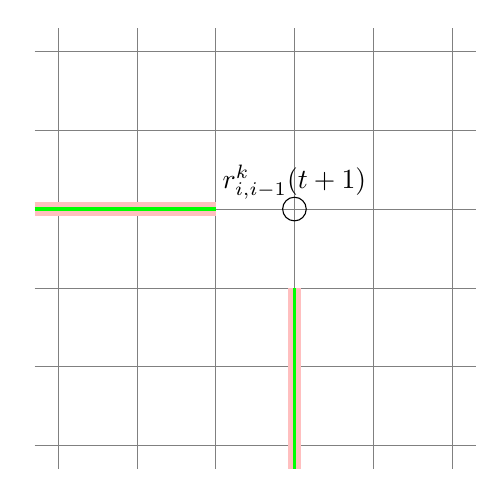
\begin{tikzpicture}[scale=1]
\draw[step=1cm,gray,very thin] (-0.3,-0.3) grid (5.3,5.3);
\draw [pink, line width=5pt](-0.3,3)--(2,3);
\draw [pink, line width=5pt](3,-0.3)--(3,2);
\draw [green, very thick](-0.3,3)--(2,3);
\draw [green,very thick](3,-0.3)--(3,2);

\draw (3,3) circle [radius=0.15];
\node [above, black] at (3,3) {$r_{i,i-1}^k(t+1)$};

\end{tikzpicture}

One can see that $L_{1}^{k}\left(t\right)=L_{1}^{k}\left(t+1\right)$
and hence $\Phi_{1}^{k}\left(t\right)\subseteq\Phi_{1}^{k}\left(t+1\right)$
also $\Phi_{0}^{k}\left(t\right)^{+}\cap L_{1}^{k}\left(t+1\right)=\varnothing$
these two gives:
\[
a_{1}^{k}\left(t\right)+\varphi_{1}^{k}\left(t\right)=\varphi_{1}^{k}\left(t\right)\leq\varphi_{1}^{k}\left(t+1\right)=\varphi_{1}^{k}\left(t+1\right)+p_{1}^{k}\left(t+1\right)\leq\varphi_{1}^{k}\left(t+1\right)+p_{1}^{k}\left(t+1\right)+f_{1}^{k}\left(t+1\right).
\]

Case 2: $\Delta r_{0}^{k}\left(t\right)=1$ but $\Delta_{1}^{k}\left(t\right)=0$,
therefore $a_{1}^{k}\left(t\right)=0$. Look at:

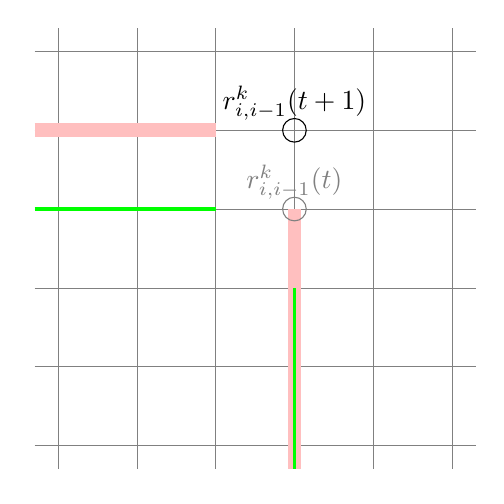
\begin{tikzpicture}[scale=1]
\draw[step=1cm,gray,very thin] (-0.3,-0.3) grid (5.3,5.3);
\draw [pink, line width=5pt](-0.3,4)--(2,4);
\draw [pink, line width=5pt](3,-0.3)--(3,3);
\draw [green, very thick](-0.3,3)--(2,3);f
\draw [green,very thick](3,-0.3)--(3,2);
%\draw [olive,very thick,dashed](0,4)--(5,4);

\draw [gray](3,3) circle [radius=0.15];
\node [above, gray] at (3,3) {$r_{i,i-1}^k(t)$};
\draw (3,3+1) circle [radius=0.15];
\node [above, black] at (3,3+1) {$r_{i,i-1}^k(t+1)$};

\end{tikzpicture}

One can see that if $p_{10}^{k}\left(t+1\right)=-1$ then $\Phi_{0}^{k}\left(t\right)^{+}\cap L_{1}^{k}\left(t\right)\ne\varnothing$
and there is a fire at the rightest point of $L_{0}^{k}\left(t\right)$
and hence at the top point of $L_{1}^{k}\left(t+1\right)$ so $1+\varphi_{1}^{k}\left(t\right)\leq\varphi_{1}^{k}\left(t+1\right)$
and hence
\[
a_{1}^{k}\left(t\right)+\varphi_{1}^{k}\left(t\right)=\left(\varphi_{1}^{k}\left(t\right)+1\right)-1\leq\varphi_{1}^{k}\left(t+1\right)-1=\varphi_{1}^{k}\left(t+1\right)+p_{10}^{k}\left(t+1\right)\leq\varphi_{1}^{k}\left(t+1\right)+p_{10}^{k}\left(t+1\right)+f_{1}^{k}\left(t+1\right).
\]

Case 3: $\Delta r_{0}^{k}\left(t\right)=\Delta r_{1}^{k}\left(t\right)=1$

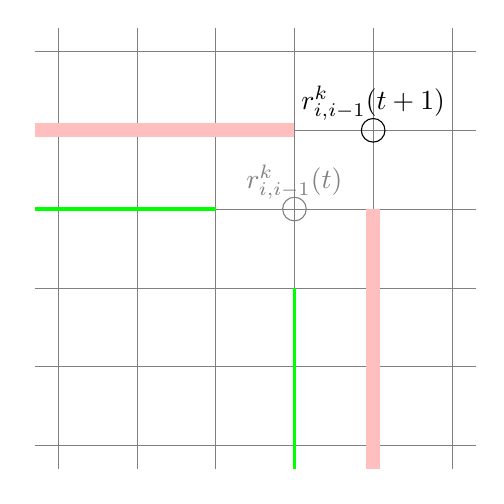
\begin{tikzpicture}[scale=1]
\draw[step=1cm,gray,very thin] (-0.3,-0.3) grid (5.3,5.3);
\draw [pink, line width=5pt](-0.3,4)--(3,4);
\draw [pink, line width=5pt](4,-0.3)--(4,3);
\draw [green, very thick](-0.3,3)--(2,3);
\draw [green,very thick](3,-0.3)--(3,2);
%\draw [olive,very thick,dashed](0,4)--(5,4);

\draw [gray](3,3) circle [radius=0.15];
\node [above, gray] at (3,3) {$r_{i,i-1}^k(t)$};
\draw (3+1,3+1) circle [radius=0.15];
\node [above, black] at (3+1,3+1) {$r_{i,i-1}^k(t+1)$};

\end{tikzpicture}

One can see that $\Phi_{1}^{k}\left(t\right)^{+}\cap L_{0}^{k}\left(t+1\right)=\varnothing$
so $p_{1}^{k}\left(t+1\right)=0$. if $\Phi_{1}^{k}\left(t\right)$
is non empty then is has $\left|\Phi_{1}^{k}\left(t\right)\right|+1$
neighbors in $L_{1}^{k}\left(t+1\right)$ therefore 
\[
\varphi_{1}^{k}\left(t\right)+a_{1}^{k}\left(t\right)=\varphi_{1}^{k}\left(t\right)+1\leq\varphi_{1}^{k}\left(t+1\right)+f_{1}^{k}\left(t+1\right)=\varphi_{1}^{k}\left(t+1\right)+f_{1}^{k}\left(t+1\right)+p_{1}^{k}\left(t+1\right)
\]
, if $\Phi_{1}^{k}\left(t\right)$ is empty then $a_{1}^{k}\left(t\right)=0,\varphi_{1}^{k}\left(t\right)=0$
and hence
\[
\varphi_{1}^{k}\left(t\right)+a_{1}^{k}\left(t\right)=0=p_{1}^{k}\left(t+1\right)\leq p_{1}^{k}\left(t+1\right)+\varphi_{1}^{k}\left(t+1\right)+f_{1}^{k}\left(t+1\right).
\]

Case 4: $\Delta r_{0}^{k}\left(t\right)=0$ and $\Delta r_{1}^{k}\left(t\right)=1$

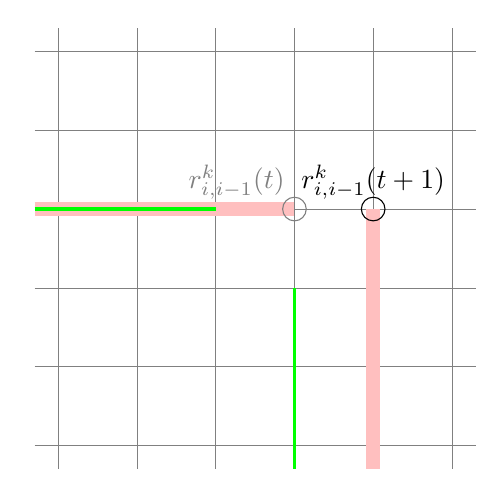
\begin{tikzpicture}[scale=1]
\draw[step=1cm,gray,very thin] (-0.3,-0.3) grid (5.3,5.3);
\draw [pink, line width=5pt](-0.3,3)--(3,3);
\draw [pink, line width=5pt](4,-0.3)--(4,3);
\draw [green, very thick](-0.3,3)--(2,3);
\draw [green,very thick](3,-0.3)--(3,2);

\draw [gray](3,3) circle [radius=0.15];
\node [above left , gray] at (3,3) {$r_{i,i-1}^k(t)$};
\draw (3+1,3) circle [radius=0.15];
\node [above , black] at (3+1,3) {$r_{i,i-1}^k(t+1)$};

\end{tikzpicture}

First, $\Phi_{1}^{k}\left(t\right)=\varnothing$ implies $a_{1}^{k}\left(t\right)=\varphi_{1}^{k}\left(t\right)=0$
, use non negativity of $\varphi_{1}^{k}\left(t+1\right),f_{1}^{k}\left(t+1\right),p_{1}^{k}\left(t+1\right)$
to obtain 
\[
\varphi_{1}^{k}\left(t\right)+a_{1}^{k}\left(t\right)=0\leq1=p_{1}^{k}\left(t+1\right)\leq p_{1}^{k}\left(t+1\right)+\varphi_{1}^{k}\left(t+1\right)+f_{1}^{k}\left(t+1\right).
\]
 If $\Phi_{1}^{k}\left(t\right)^{+}\cap L_{0}^{k}\left(t+1\right)\ne\varnothing$
then $\Phi_{1}^{k}\left(t\right)$ has only $\varphi_{1}^{k}\left(t\right)$
neighbors in $L_{1}^{k}\left(t+1\right)$ but $p_{1}^{k}\left(t+1\right)=1$
and hence 
\[
\varphi_{1}^{k}\left(t\right)\leq\varphi_{1}^{k}\left(t+1\right)+f_{1}^{k}\left(t+1\right),
\]
use $p_{1}^{k}\left(t+1\right)=1$ to conclude
\[
a_{1}^{k}\left(t\right)+\varphi_{1}^{k}\left(t\right)\leq1+\varphi_{1}^{k}\left(t\right)\leq\varphi_{1}^{k}\left(t+1\right)+f_{1}^{k}\left(t+1\right)+p_{1}^{k}\left(t+1\right).
\]

All these argument are for the $0,1$ corner, use the same arguments
to earn growth from the $1,2$ corner and conclude that
\[
2a_{1}^{k}\left(t\right)+\varphi_{1}^{k}\left(t\right)\leq\varphi_{1}^{k}\left(t+1\right)+f_{1}^{k}\left(t+1\right)+p_{1}^{k}\left(t+1\right).
\]
\end{proof}

\section{Upper bound}

Let $S$ be an initial fire then there is $r$ such that the initial
fire contained in $\left[-r,r\right]^{2}\times\left[h\right]$. The
amount of firefighters satisfies $f\left(t\right)^{\ast}=cht>3ht$,
denote $c=3+\varepsilon$.

The strategy is symmetric in all levels, the following description
is for one level and $f^{k}\left(t\right)^{\ast}=ct$.

\paragraph{Phase one:}

From time $1$ until time $t_{1}=2r+1$: 

Place all the $c\left(2r+1\right)>6r+3$ firefighters on the line:
$\left[-3r+1,3r+1\right]\times\left\{ 3r+1\right\} $

On phase one, at time $t$ fire bounded at $y=r+t-1$ and $x_{\min}=-\left(r+t-1\right),x_{\max}=r+t-1$.

\noindent\begin{minipage}[t]{1\columnwidth}%
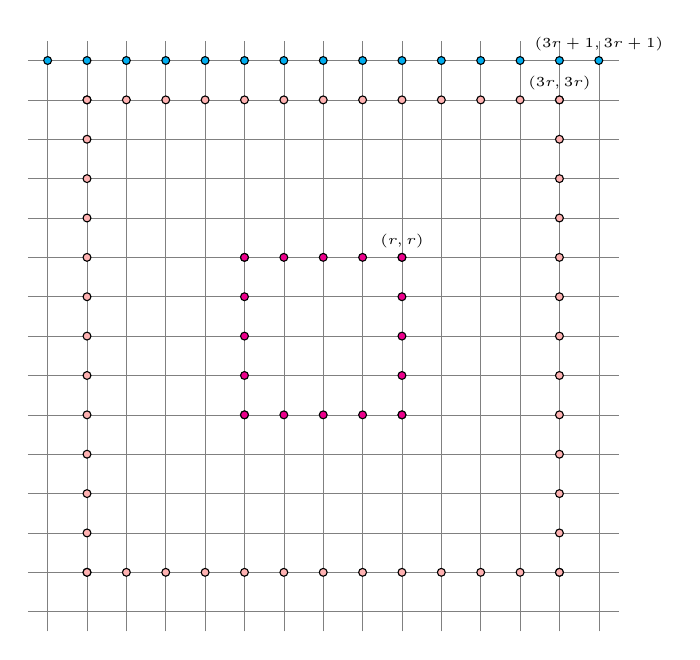
\begin{tikzpicture} [scale=0.5]

\draw [step=1cm,gray, very thin] (-7.5,-7.5) grid (7.5,7.5);

\foreach \y in {-6,...,6}
\foreach \x in {-6,6}
{
	\draw [fill=red!30!white] (\x,\y) circle [radius =0.1];
}
\foreach \y in {-6,6}
\foreach \x in {-6,...,6}
{
	\draw [fill=red!30!white] (\x,\y) circle [radius =0.1];
}


\foreach \x in {-2,...,2}
\foreach \y in {-2,2}
{
	\draw [fill=magenta] (\x,\y) circle [radius =0.1];
}
\foreach \x in {-2,2}
\foreach \y in {-2,...,2}
{
	\draw [fill=magenta] (\x,\y) circle [radius =0.1];
}

\draw (2,2) node [above] {\tiny $(r,r)$};


\draw (6,6) node [above] {\tiny $(3r,3r)$};

\foreach \x in {-7,...,7}
{
	\draw [fill=cyan] (\x,7) circle [radius =0.1];
}
\draw (7,7) node [above] {\tiny $(3r+1,3r+1)$};


\end{tikzpicture}%
\end{minipage}

\paragraph{Phase two}

From time $2r+2$ until $t_{2}=2r+1+6r\left\lceil \frac{1}{\varepsilon}\right\rceil $,
a duration of $6r\left\lceil \frac{1}{\varepsilon}\right\rceil $
turns.

Each turn place two firefighters on the line $y=\left\{ 3r+1\right\} $
to maintain the north front. The east front bounded by $\left\{ \left(3r+\left(t-t_{1}\right)\right)\right\} \times\left[3r,-\left(3r+\left(t-t_{1}\right)\right)\right]$
and hence at time $t_{2}$ place all the remaining $\left(1+\varepsilon\right)6r\left\lceil \frac{1}{\varepsilon}\right\rceil \geq6r\left\lceil \frac{1}{\varepsilon}\right\rceil +6r$
firefighters on the line 
\[
\left\{ \left(3r+6r\left\lceil \frac{1}{\varepsilon}\right\rceil +1\right)\right\} \times\left[3r,-\left(3r+6r\left\lceil \frac{1}{\varepsilon}\right\rceil \right)+1\right].
\]

\noindent\begin{minipage}[t]{1\columnwidth}%
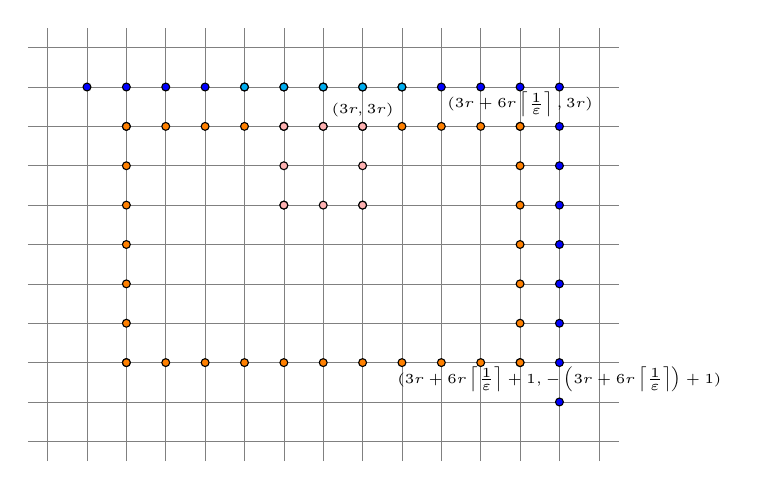
\begin{tikzpicture} [scale=0.5]

\draw [step=1cm,gray, very thin] (-7.5,-7.5) grid (7.5,3.5);

\foreach \y in {-5,...,1}
\foreach \x in {-5,5}
{
	\draw [fill=orange] (\x,\y) circle [radius =0.1];
}
\foreach \y in {-5,1}
\foreach \x in {-5,...,5}
{
	\draw [fill=orange] (\x,\y) circle [radius =0.1];
}

\draw (5,1) node [above] {\tiny $(3r+6r\left\lceil \frac{1}{\varepsilon}\right\rceil ,3r)$};


\foreach \x in {-1,...,1}
\foreach \y in {-1,1}
{
	\draw [fill=red!30!white] (\x,\y) circle [radius =0.1];
}
\foreach \x in {-1,1}
\foreach \y in {-1,...,1}
{
	\draw [fill=red!30!white] (\x,\y) circle [radius =0.1];
}

\draw (1,1) node [above] {\tiny $(3r,3r)$};


\foreach \x in {-6,...,6}
{
	\draw [fill=blue] (\x,2) circle [radius =0.1];
}
\foreach \y in {-6,...,1}
{
	\draw [fill=blue] (6,\y) circle [radius =0.1];
}
\draw (6,-6) node [above] {\tiny $(3r+6r\left\lceil \frac{1}{\varepsilon}\right\rceil +1,-\left(3r+6r\left\lceil \frac{1}{\varepsilon}\right\rceil \right)+1)$};

\foreach \x in {-2,...,2}
{
	\draw [fill=cyan] (\x,2) circle [radius =0.1];
}


\end{tikzpicture}%
\end{minipage}

\paragraph{Phase three}

...

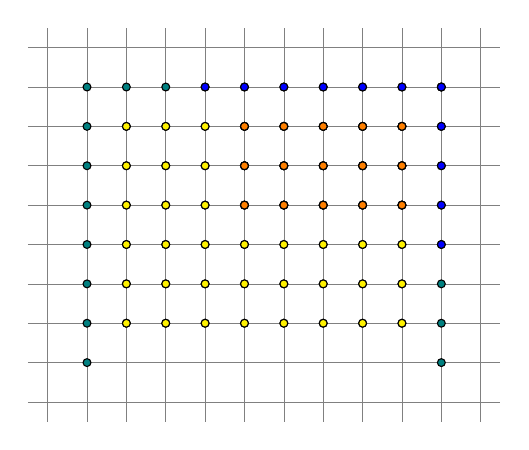
\begin{tikzpicture} [scale=0.5]

\draw [step=1cm,gray, very thin] (-7.5,-6.5) grid (4.5,3.5);

\foreach \x in {-5,...,2}
\foreach \y in {-4,...,1}
{
	\draw [fill=yellow] (\x,\y) circle [radius =0.1];
}
\foreach \x in {-5,...,2}
\foreach \y in {-4,...,1}
{
	\draw [fill=yellow] (\x,\y) circle [radius =0.1];
}

\foreach \x in {-6,...,3}
\foreach \y in {2}
{
	\draw [fill=teal] (\x,\y) circle [radius =0.1];
}
\foreach \x in {-6,3}
\foreach \y in {-5,...,1}
{
	\draw [fill=teal] (\x,\y) circle [radius =0.1];
}



\foreach \x in {-2,...,2}
\foreach \y in {-1,...,1}
{
	\draw [fill=orange] (\x,\y) circle [radius =0.1];
}
\foreach \x in {-2,...,2}
\foreach \y in {-1,...,1}
{
	\draw [fill=orange] (\x,\y) circle [radius =0.1];
}


\foreach \y in {-2,...,2}
{
	\draw [fill=blue] (3,\y) circle [radius =0.1];
}
\foreach \x in {-3,...,3}
{
	\draw [fill=blue] (\x,2) circle [radius =0.1];
}

\end{tikzpicture}

\paragraph{Phase four}

...

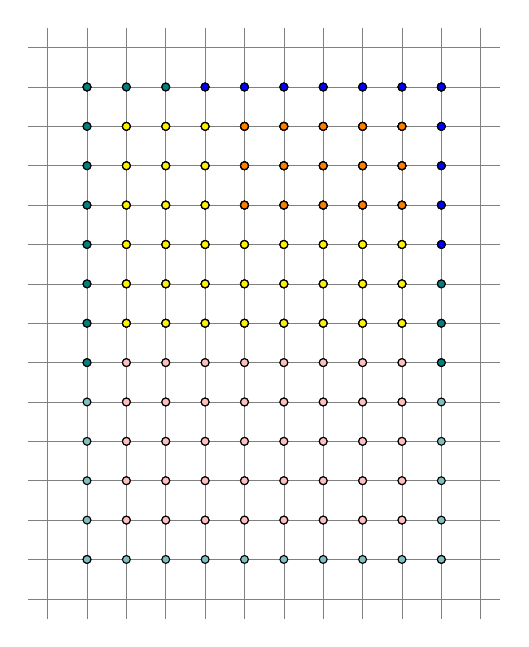
\begin{tikzpicture} [scale=0.5]

\draw [step=1cm,gray, very thin] (-7.5,-11.5) grid (4.5,3.5);

\foreach \x in {-5,...,2}
\foreach \y in {-9,...,1}
{
	\draw [fill=pink] (\x,\y) circle [radius =0.1];
}
\foreach \x in {-5,...,2}
\foreach \y in {-9,...,1}
{
	\draw [fill=pink] (\x,\y) circle [radius =0.1];
}

\foreach \x in {-6,...,3}
\foreach \y in {-10,2}
{
	\draw [fill=teal!50!white] (\x,\y) circle [radius =0.1];
}
\foreach \x in {-6,3}
\foreach \y in {-10,...,2}
{
	\draw [fill=teal!50!white] (\x,\y) circle [radius =0.1];
}


\foreach \x in {-5,...,2}
\foreach \y in {-4,...,1}
{
	\draw [fill=yellow] (\x,\y) circle [radius =0.1];
}
\foreach \x in {-5,...,2}
\foreach \y in {-4,...,1}
{
	\draw [fill=yellow] (\x,\y) circle [radius =0.1];
}


\foreach \x in {-6,...,3}
\foreach \y in {2}
{
	\draw [fill=teal] (\x,\y) circle [radius =0.1];
}
\foreach \x in {-6,3}
\foreach \y in {-5,...,1}
{
	\draw [fill=teal] (\x,\y) circle [radius =0.1];
}



\foreach \x in {-2,...,2}
\foreach \y in {-1,...,1}
{
	\draw [fill=orange] (\x,\y) circle [radius =0.1];
}
\foreach \x in {-2,...,2}
\foreach \y in {-1,...,1}
{
	\draw [fill=orange] (\x,\y) circle [radius =0.1];
}


\foreach \y in {-2,...,2}
{
	\draw [fill=blue] (3,\y) circle [radius =0.1];
}
\foreach \x in {-3,...,3}
{
	\draw [fill=blue] (\x,2) circle [radius =0.1];
}



\end{tikzpicture}	
\begin{thebibliography}{1}
\bibitem{FH} Ohad N. Feldheim, Rani Hod, 3/2 Firefighters are
not enough.

\bibitem{key-2} P. Fogarty, Catching the fire on grids, M.Sc. Thesis,
University of Vermont, 2003.

\bibitem{key-3} Gideon Amir, Rangel Baldasso \& Gady Kozma. The firefighter
problem on polynomial and intermediate growth groups, 2020.
\end{thebibliography}

\end{document}